\documentclass[11pt, a4paper]{article}

\usepackage[pdftex,colorlinks=true,
                       pdfstartview=FitV,
                       linkcolor=blue,
                       citecolor=blue,
                       urlcolor=blue
           ]{hyperref}

\usepackage{amssymb}
\usepackage{amsmath}
\usepackage{graphicx}
\usepackage{url}
\usepackage{wrapfig}
\usepackage{fancyvrb}
\fvset{fontsize=\small, frame=lines}

\newcommand{\BB}{\textsc{B{\small\&}B}}
\newcommand{\DRS}{\textsc{drs}}
\newcommand{\DRT}{\textsc{drt}}
\newcommand{\FOL}{\textsc{fol}}
\newcommand{\LF}{\textsc{lf}}
\newcommand{\NLP}{\textsc{nlp}}
\newcommand{\NLTK}{\textsc{nltk}}
\newcommand{\RTE}{\textsc{rte}}


\pdfinfo{
   /Author 		(Dan Garrette and Ewan Klein)
   /Title  		(An Extensible Toolkit for Computational Semantics)
   /Subject 		(Computational Semantics)
   /Keywords 		(Natural Language Processing;Computational Semantics;Natural Language Toolkit;NLTK)
}

\usepackage[round]{natbib}
% \bibpunct{[}{]}{;}{a}{,}{,}
\bibliographystyle{plainnat}

\usepackage{lingmacros}

%%%%%%%%%%%%%%%%%%%%%%%%%%%
% Copied from covington.sty by Michael A. Covington
%%%%%%%%%%%%%%%%%%%%%%%%%%%
\newcommand{\dhgdrs}[2]
{
    {
    \it
    \begin{tabular}{|l|}
    \hline
    ~ \vspace{-2ex} \\
    #1
    \\
    ~ \vspace{-2ex} \\
    \hline
    ~ \vspace{-2ex} \\
    #2
    \\
    ~ \\    % can't vspace here or the line will come out wrong
    \hline
    \end{tabular}
    }
}
\newcommand{\dhgsdrs}[3]
{\begin{tabular}{l}
\mbox{\it #1} \\
~ \\
\dhgdrs{#2}{#3}
\end{tabular}}\newcommand{\dhgifdrs}[4]
{
  \mbox{\dhgdrs{#1}{#2}~~{\large $\Rightarrow$}~\dhgdrs{#3}{#4}}
}
\newcommand{\dhgalifdrs}[4]
{
  \mbox{$\!\!\!$\dhgdrs{#1}{#2}~~{\large $\Rightarrow$}~\dhgdrs{#3}{#4}}
}
\newcommand{\dhgnegdrs}[2]
{
  \mbox{{\large $\neg$}\dhgdrs{#1}{#2}}
}
%%%%%%%%%%%%%%%%%%%%%%%%%%%
% END covington.sty
%%%%%%%%%%%%%%%%%%%%%%%%%%%


\begin{document}


\title{An Extensible Toolkit for Computational Semantics}
\author{Dan Garrette \and Ewan Klein}
\date{\today}

\maketitle

\section{Introduction}

In this paper we focus on the software for computational semantics provided
by the Python-based Natural Language Toolkit (\NLTK). The semantics
modules in \NLTK\ are
inspired in large part by the approach developed in \citet{BB}
(henceforth referred to as \BB).
Since Blackburn and Bos have also provided a software suite to
accompany their excellent textbook, one might ask what the
justification is for the \NLTK\ offering, which is similarly slanted
towards teaching computational semantics.

This question can be answered in a number of ways. First, we believe
there is intrinsic merit in the availability of different software
tools for semantic analysis, even when there is some duplication of
coverage; and this will become more true as computational semantics
starts to be as widely studied as computational syntax. For example, 
one rarely hears the objection that too many implementations of 
syntactic parsers are available.  Moreover, the \NLTK\ software 
significantly goes beyond \BB\ in providing an implementation of 
Glue Semantics.

Second, whatever the relative merits of Prolog vs.\ Python as
programming languages, there is surely an advantage in offering
students and instructors a choice in this respect. Given that many
students have either already been exposed to Java, or else have had no
programming experience at all, Python offers them the option of
accomplishing interesting results with only a shallow
learning curve.

Third, \NLTK\ is a rapidly developing, open source
project\footnote{See \url{http://www.nltk.org}} with a broad coverage of
natural language processing (\NLP) tools; see \citet{Multidisciplinary} for
a recent overview. This wide functionality has a number of benefits,
most notably that lexical, syntactic and semantic processing can be
carried out within a uniform computational framework. As a result,
\NLTK\ makes it much easier to include some computational semantics
subject matter in
a broad course on natural language analysis, rather than having to
devote a whole course exclusively to the topic.

Fourth, \NLTK\ is accompanied by a substantial collection of corpora,
plus easy-to-use corpus readers.  This collection, which currently
stands at 45 corpora, includes parsed, POS-tagged, plain text,
categorized text, and
lexicons.\footnote{\url{http://www.nltk.org/corpora.html}} The
availability of corpora can help encourage students to go beyond
writing toy grammars, and instead to start grappling with the
complexities of semantically analysing realistic bodies of text.

Fifth, \NLTK\ is not just for students. Although Python is slower than
languages like Java and C++, its suitability for rapid prototyping
makes it an attractive addition to the researcher's inventory of
resources. Building an experimental set-up in \NLTK\ to test a
hypothesis or explore some data is straightforward and quick, and the
rich variety of existing \NLP\ components in the toolkit allows rapid
assembly of quite sophisticated processing pipelines.


\section{Overview}
\label{sec:overview}


\begin{wrapfigure}{r}{3in}
%\label{modules}
  \centering
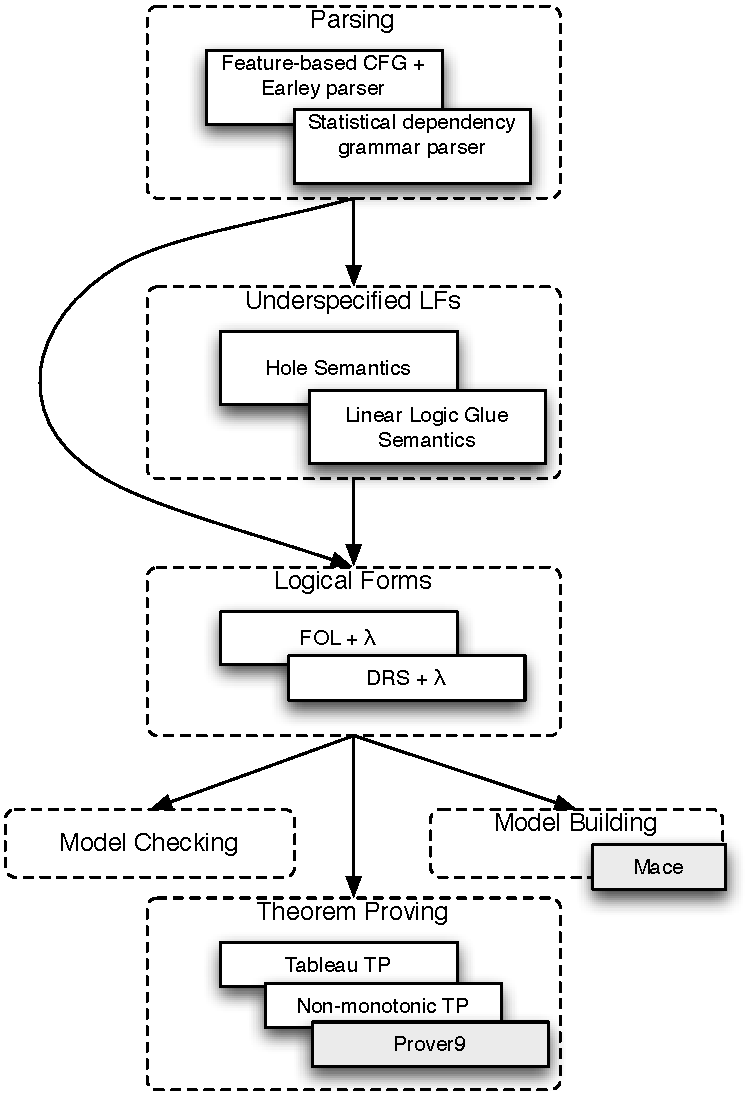
\includegraphics[scale=.6]{modules}  
%  \caption{Overview of semantic processing in NLTK}
\end{wrapfigure}

Like \BB, we assume that one of the most important tasks for
the teacher is to ground students in the basic concepts of first order
logic and the lambda calculus, model-theoretic interpretation and
inference. This provides a basis for exploring more modern approaches
like Discourse Representation Theory (\DRT; \citet{KampReyle}) and
underspecification.

In the accompanying figure, we give a diagrammatic overview of the
main semantics-related functionality that is currently available in
\NLTK.  Logical forms (\LF s) can be induced as result of syntactic
parsing, using either feature-based grammars that are processed with
an Earley chart parser, or else by associating \LF s with the output
of a broad-coverage dependency parser. Our basic \LF s are expressions
of first order logic, supplemented with the lambda operator. However,
we also admit Discourse Representation Structures (\DRS s) as \LF s,
and underspecified \LF s can be built using either Hole Semantics
\citep{BB} or Glue Semantics
\citep{Dalrymple:1999:RRB}. 
%\citep{Dalrymple:1999:RRB,Dalrymple2001}. 
Once we have constructed \LF
s, they can be evaluated in a first order model \citep{Klein06altw},
tested for equivalence and validity in a variety of theorem provers,
or tested for consistency in a model builder. The latter two tasks are
aided by \NLTK\
 interfaces to third-party inference tools, currently Prover9
and Mace4 \citep{McCune}.

We do not have space in this paper to discuss all of these components,
but will try to present some of the key aspects, and along the way
noting certain points of difference \textit{vis-\`a-vis} \BB.


\section{Logical Form}

\subsection{First Order Predicate Logic with Lambda Calculus}
From a pedagogical point of view, it is usually important to ensure
that students have some grasp of the language of first order predicate
logic (\FOL), and can also manipulate $\lambda$-abstraction.  The
\texttt{nltk.sem.logic} module contains an object-oriented approach
to representing \FOL\ plus
$\lambda$-abstraction. Logical formulas are typically fed to the
\texttt{logic} parser as strings, and then represented as instances of
various subclasses of \texttt{Expression}, as we will see shortly.

An attractive feature of Python is its interactive interpreter,
which allows the user to enter Python expressions and statements for
evaluation. In the example below and subsequently, \verb!>>>! is the
Python interpreter's prompt. 
\begin{Verbatim}[numbers=left]
>>> from nltk.sem import logic
>>> lp = logic.LogicParser()
>>> e = lp.parse('all x.(girl(x) -> exists y.(dog(y) & chase(x,y)))')
>>> e
<AllExpression all x.(girl(x) -> exists y.(dog(y) & chase(x,y)))>
\end{Verbatim}
As illustrated, the result of parsing the formula at line~3 is an object
\texttt{e} belonging to the class \texttt{AllExpression}, itself a
subclass of \texttt{Expression}.  All such subclasses have numerous
methods that implement standard logical operations. For
example, the \texttt{simplify()} method carries out
$\beta$-conversion; the \texttt{free()} method finds
all the free variables in an expression; and for quantified expressions
(such as \texttt{AllExpression}s), there is an \texttt{alpha\_convert()}
method.  The \texttt{logic}
module will $\alpha$-convert automatically when appropriate to
avoid name-clashes in the \texttt{replace()} method. Let's illustrate
these methods
with a formula involving $\lambda$-abstraction, namely
\verb!\x.P(x)(y)!; we use \protect{\verb!\!} to represent
$\lambda$. (Since \verb!\! is a special character in Python,
we add the \texttt{r} prefix to strings containing it to preclude
additional escape characters.)
\begin{Verbatim}
>>> from nltk.sem import Variable
>>> e1 = lp.parse(r'\x.P(x)(y)')
>>> print e1.simplify()
P(y)
>>> e2 = lp.parse('all x.P(x,a,b)')
>>> print e2.free()
set([<Variable('a'), Variable('b')])
>>> print e2.alpha_convert(Variable('z'))
all z.P(z,a,b)
>>> e3 = lp.parse('x')
>>> print e2.replace(Variable('b'), e3)
all z1.P(z1,a,x)
\end{Verbatim}
% A feature of Python that lends itself well to working with logical
% expressions is its operator overloading.  The operators \texttt{-},
% \texttt{\&}, \texttt{$|$}, \texttt{$>$}, \texttt{$<$} can be used
% for \emph{negation}, \emph{conjunction}, \emph{disjunction},
% \emph{implication}, and \emph{biconditional}, respectively.  The
% parenthesis of a function call are overloaded to perform function
% application.  Python's built-in \texttt{lambda} operator can also be
% used with logical expressions because it uses function calls.
% \begin{Verbatim}
% >>> P = parser.parse('P')
% >>> x = parser.parse('x')
% >>> y = parser.parse('y')
% >>> print P(x) & P(y)
% (P(x) & Q(y))
% >>> print (lambda x: P(x))(y)
% P(y)
% \end{Verbatim}
Allowing students to build simple first order models, and evaluate
expressions in those models, can be useful for helping them clarify
their intuitions about quantification. In the next example, we show
one of the available methods in \NLTK\ for specifying a model and
using it to determine the set of satisfiers of the open formula
$\exists x.(\mathit{girl}(y) \wedge
\mathit{chase}(x,y))$.\footnote{The triple quotes \texttt{"""} in
  Python allow us to break a logical line across several physical
  lines.},
\footnote{Given a valuation \texttt{val}, the property
  \texttt{val.domain} returns the set of all domain individuals
  specified in the valuation.}
\begin{Verbatim}
>>> from nltk.sem import parse_valuation, Model, Assignment
>>> v = """
... suzie => s
... fido => f
... rover => r
... girl => {s}
... chase => {(f, s), (r, s), (s, f)}
... """
>>> val = parse_valuation(v) #create a Valuation
>>> m = Model(val.domain, val) #initialize a Model
>>> g = Assignment(val.domain) #initialize an Assignment
>>> e4 = lp.parser('exists y. (girl(y) & chase(x, y))')
>>> m.satisfiers(e4, 'x', g) #check satisfiers of e4 wrt to x
set(['r', 'f'])
\end{Verbatim}

In \BB, $\lambda$-abstracts are second-class citizens, used
exclusively as a `glue' mechanism for composing meaning
representations. Although we use $\lambda$-abstracts as glue too,
abstracts over individual variables are interpreted in \NLTK, namely as
characteristic functions.

\texttt{Expression}s in \NLTK\ can be optionally typed (using
Montague-style types) by passing the parameter \texttt{type\_check=True} to
\texttt{LogicParser}.  Apart from allowing the user to display the
\texttt{Expression}'s type with \texttt{gettype()}, type checking will
raise an exception for non-well typed expressions:
\begin{Verbatim}
>>> tlp = logic.LogicParser(type_check=True)
>>> a = tlp.parse(r'\x y.sees(x,y)')
>>> a.gettype()
<e,<e,t>>
>>> b = tlp.parse(r'\x y.see(x,y)(\x.man(x))')
Traceback (most recent call last):
  . . .
TypeException: The function '\x y.see(x,y)' is of type '<e,<e,t>>' 
and cannot be applied to '\x.man(x)' of type '<e,t>'.  Its argument 
must be of type 'e'.
\end{Verbatim}
% Fix for code colorization: >>>>

\subsection{Discourse Representation Theory}
As mentioned earlier, \NLTK\ contains an extension to the
\texttt{logic} module for working with Discourse Representation Theory
(\DRT) \citep{KampReyle}.  The \texttt{nltk.sem.drt} module introduces
a \texttt{DRS()} constructor which takes lists of discourse referents
and conditions as initialization parameters:
\vspace{-2ex}
\enumsentence{\label{drt3} \texttt{DRS([j,d],[John(j), dog(d),
    sees(j,d)])}} 

On top of the functionality available for \FOL\
expressions, \DRT\ expressions have a `\DRS-concatenation' operator,
represented as the \texttt{+} symbol.  The concatenation of two \DRS s
is a single \DRS\ containing the merged discourse referents and the
conditions from both arguments.  \DRS-concatenation automatically
$\alpha$-converts bound variables to avoid name-clashes.  The
\texttt{+} symbol is overloaded so that \DRT\ expressions can be added
together easily.  The \texttt{nltk.sem.drt} parser allows \DRS s to be
specified succinctly as strings.
\begin{Verbatim}
>>> from nltk.sem import drt
>>> dp = drt.DrtParser()
>>> d1 = dp.parse('([x],[walk(x)]) + ([y],[run(y)])')
>>> print d1
(([x],[walk(x)]) + ([y],[run(y)]))
>>> print d1.simplify()
([x,y],[walk(x), run(y)])
>>> d2 = dp.parse('([x,y],[Bill(x), Fred(y)])')
>>> d3 = dp.parse("""([],[([u],[Porsche(u), own(x,u)])
...  ->  ([v],[Ferrari(v), own(y,u)])])""")
>>> d4 = d2 + d3
>>> print d4.simplify()
([x,y],[Bill(x), Fred(y),
(([u],[Porsche(u), own(x,u)]) -> ([v],[Ferrari(v), own(y,u)]))])
\end{Verbatim}

\noindent
\DRT\ expressions can be converted to their first order predicate
logic equivalents using the \texttt{toFol()} method and can be
graphically rendered on screen with the \texttt{draw()} method.

\begin{wrapfigure}{r}{0.2\textheight}
\vspace{-16ex}
\begin{center}
   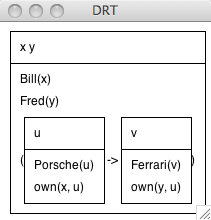
\includegraphics[scale=.5]{drs.png}
 \end{center}
\vspace{-4ex}
\caption{\small DRS Screenshot} 
\vspace{-10ex}
\end{wrapfigure}

\begin{Verbatim}[frame=none]
>>> print d1.toFol()
(exists x.walk(x) & exists y.run(y))
>>> d4.simplify().draw()
\end{Verbatim}

Since the $\lambda$ operator can be combined with \DRT\ expressions,
the \texttt{nltk.sem.drt} module can be used as a plug-in replacement for 
\texttt{nltk.sem.logic} in building compositional semantics.


\section{Scope Ambiguity and Underspecification}

Two key questions in introducing students to computational semantics are:
\begin{enumerate}
\item[Q1:] How are semantic representations constructed from input
  sentences?
\vspace{-2ex}
\item[Q2:] What is scope ambiguity and how is it captured?
\end{enumerate}
A standard pedagogical approach is to address (Q1) with a simple
syntax-driven induction of logical forms which fails to deal with
scope ambiguity, while (Q2) is addressed by introducing underspecified
representations which are resolved to produce different readings of
ambiguous sentences.

\NLTK\ includes a suite of parsing tools, amongst which is a chart
parser for context free grammars augmented with feature structures. A
`semantics' feature \texttt{sem} allows us to compose the
contributions of constituents to build a logical form for a complete
sentence.  To illustrate, the following minimal grammar
\texttt{sem1.fcfg} handles quantification and intransitive verbs
(where values such as \texttt{?subj} and \texttt{?vp} are unification
variables, while \texttt{P} and \texttt{Q} are $\lambda$-bound object
language variables):
\begin{Verbatim}
S[sem = <?subj(?vp)>] -> NP[sem=?subj] VP[sem=?vp]
VP[sem=?v] -> IV[sem=?v]
NP[sem=<?det(?n)>] -> Det[sem=?det] N[sem=?n]
Det[sem=<\P.\Q.exists x.(P(x) & Q(x))>] -> 'a'
N[sem=<\x.dog(x)>] -> 'dog'
IV[sem=<\x.bark(x)>] -> 'barks'
\end{Verbatim}
Using \texttt{sem1.fcfg}, we can parse \textit{A dog barks} and view
its semantics. 
%  It should be noted that if the
% \texttt{load\_earley()} method's argument \texttt{trace} is set to a
% positive number, then the parser prints detailed information showing
% how the sentence was parsed.  
The \texttt{load\_earley()} method
takes an optional parameter \texttt{logic\_parser} which specifies the
logic-parser for processing the value of the \texttt{sem} feature, thus
allowing different kinds of logical forms to be constructed.
\begin{Verbatim}
>>> from nltk.parse import load_earley
>>> parser = load_earley('grammars/sem1.fcfg', trace=0)
>>> trees = parser.nbest_parse('a dog barks'.split())
>>> print trees[0].node['sem'].simplify()
exists x.(dog(x) & bark(x))
\end{Verbatim}

Underspecified logical forms allow us to loosen the relation between
syntactic and semantic representations. We consider two approaches to
underspecification, namely Hole
Semantics and Glue Semantics. Since the former will be familiar from 
\BB, we devote most of our attention to presenting Glue
Semantics.

\subsection{Hole Semantics}

Hole Semantics in \NLTK\ is handled by the
\texttt{nltk.sem.hole} module, which uses a context free grammar to
generate an underspecified logical form.  Since the latter is itself a
formula of first order logic, we can continue to use the \texttt{sem} feature
in the context free grammar:
\begin{Verbatim}[frame=none,fontsize=\small]
N[sem=<\x h l.(PRED(l,dog,x) & LEQ(l,h) & HOLE(h) & LABEL(l))>] -> 'dog'
\end{Verbatim}
The Hole Semantics module uses a standard plugging algorithm to derive the
sentence's readings from the underspecified \LF.
\begin{Verbatim}
>>> from nltk.sem import hole
>>> readings = hole.main('every girl chases a dog')
>>> for r in reading: print r
exists z1.(dog(z1) & all z2.(girl(z2) -> chase(z1,z2)))
all z2.(girl(z2) -> exists z1.(dog(z1) & chase(z1,z2)))
\end{Verbatim}


\subsection{Glue Semantics}
Glue Semantics\footnote{\url{http://nltk.googlecode.com/svn/trunk/doc/contrib/sem/index.html}}
 \citep{Dalrymple:1999:RRB}, or Glue for
short, is an approach to compositionality that tries to handle
semantic ambiguity by using resource-sensitive logic to assemble
meaning expressions.
The approach builds proofs over `meaning constructors'; these are of the
form $\cal{M}: \cal{G}$, where $\cal{M}$ is a meaning representation and
$\cal{G}$ is a term of linear logic.  The linear logic term $\cal{G}$
dictates how the meaning expression $\cal{M}$ can be combined.  Each
distinct proof that can be derived reflects a different semantic
reading of the entire sentence.

The variant of linear logic that we use has \emph{(linear)
  implication} (i.e., $\multimap$)  as its
only operator, so the primary operation during the proof is Modus
Ponens.  Linear logic is an appropriate logic to serve as `glue'
because it is resource-sensitive.  This means that when Modus Ponens
combines two terms to create a new one, the two original
terms are `consumed', and cannot be used again in the proof;
cf.\ (\ref{glue1}) vs.\ (\ref{glue2}).
Additionally, every premise must be used for the proof to be valid;
cf.\ (\ref{glue3}).
This resource-sensitivity dictates that each word contributes its
meaning exactly once to the meaning of the whole.
\newpage
\enumsentence{\label{glue1} A, (A $\multimap$ B) $\vdash$ B}
\enumsentence{\label{glue2} A, (A $\multimap$ B) $\nvdash$ A, B}
\enumsentence{\label{glue3} A, A, (A $\multimap$ B) $\nvdash$ B}
\NLTK's \texttt{nltk.gluesemantics.linearlogic} module
contains an implementation of linear logic. 

The primary rule for composing Glue formulas is (\ref{glue4}).
Function-argument application of meaning expressions is reflected (\textit{via}
the Curry-Howard isomorphism) by the application of Modus Ponens in a
linear logic proof. Note that $A$ and $B$ are meta-variables over
constants of linear logic; these constants represent `attachment
points' for meaning expressions in some kind of syntactically-derived
representation (such as an LFG \textit{f}-structure).  It is
(\ref{glue4}) which allows Glue to guide the construction of complex
meaning expressions.  
\vspace{-3ex}
\enumsentence{\label{glue4} $\alpha : A,\;
  \gamma : (A \multimap B) \vdash \gamma(\alpha) : B$} 

The \NLTK\ modules \texttt{gluesemantics.glue} and
\texttt{gluesemantics.drt\_glue} implement Glue for \FOL\ and
\DRT\ meaning expressions, respectively.
The following example shows the basic way that
Glue formulas are created and combined to derive a logical form for
\textit{John walks}: 

\begin{Verbatim}
>>> from nltk.gluesemantics.glue import GlueFormula
>>> john = GlueFormula('john', 'g')
>>> walks = GlueFormula(r'\x.walk(x)', '(g -o f)')
>>> john_walks = walks.applyto(john)
>>> print john_walks.meaning.simplify()
walk(john)
\end{Verbatim}
Thus, the non-logical constant \textit{john} is associated with the
Glue term $g$, while the meaning expression $\lambda x.walk(x)$ is
associated with $(g \multimap f)$ since it is a function that
takes $g$ as input and returns the meaning expression $f$,
corresponding to the whole
sentence.  Consequently, a proof of $f$ from the premises is a derivation
of a meaning representation for the sentence.

Scope ambiguity, resulting, for example, from quantifiers, requires the
use of \textit{variables} in the Glue terms. Such variables may be
instantiated to any linear logic constant, so long as this is carried
out uniformly. Let's assume that the quantified noun phrase
\textit{every girl} has the meaning constructor (\ref{glue5}) (where
$G$ is a linear logic variable):

\enumsentence{\label{glue5} $\lambda Q.\forall x.(girl(x) \rightarrow
  Q(x)) : ((g \multimap G) \multimap G)$}
Then the Glue derivation shown below correctly
generates two readings for the sentence \textit{Every girl chases a dog}:
\begin{Verbatim}
>>> from nltk.gluesemantics.glue import GlueFormula, Glue
>>> a = GlueFormula(r'\Q.all x.(girl(x) -> Q(x))', '((g -o G) -o G)')
>>> b = GlueFormula(r'\x y.chase(x,y)', '(g -o (h -o f))')
>>> c = GlueFormula(r'\Q.exists x.(dog(x)&Q(x))', '((h -o H) -o H)')
>>> glue = Glue()
>>> for reading in glue.get_readings(glue.gfl_to_compiled([a,b,c])):
...     print reading.simplify()
exists x.(dog(x) & all z13.(girl(z13) -> chase(z13,x)))
all x.(girl(x) -> exists z14.(dog(z14) & chase(x,z14)))
\end{Verbatim}


\section{Inference tools}
In order to perform inference over semantic representations, \NLTK\
can call both theorem provers and model builders.
The library includes a pure Python tableau-based first order theorem prover;
this is intended to allow students to study 
tableau methods for theorem proving, and provides an
opportunity for experimentation.  In addition, \NLTK\ provides
interfaces to two state-of-the-art tools, namely the theorem prover Prover9, 
and the model builder Mace4  \citep{McCune}.  % Both of these are
% powerful enough for research.

The \verb!get_prover(G, A)! method by default calls Prover9, and takes as
parameters a proof goal \texttt{G} and a list \texttt{A} of assumptions.
Here, we verify that if every dog barks, and Rover is a dog,
then it is true that Rover barks:
\begin{Verbatim}
>>> from nltk.inference import inference
>>> a = lp.parse('all x.(dog(x) -> bark(x))')
>>> b = lp.parse('dog(rover)')
>>> c = lp.parse('bark(rover)')
>>> prover = inference.get_prover(c, [a,b])
>>> prover.prove()
True
\end{Verbatim}

A theorem prover can also be used to check the logical equivalence of
expressions.  For two expressions $A$ and $B$, we can pass $(A\iff B)$
into a theorem prover and know that the theorem will be proved if and
only if the expressions are logically equivalent.  \NLTK's standard
equality operator for \texttt{Expression}s (\texttt{==}) is able to
handle situations where two expressions are identical up to
$\alpha$-conversion.  However, it would be impractical for \NLTK\ to
invoke a wider range of logic rules every time we checked for equality
of two expressions. Consequently, both the \texttt{logic} and 
\texttt{drt} modules in \NLTK\ 
have a separate method, \texttt{tp\_equals}, for checking `equality'
up to logical equivalence.
\newpage
\begin{Verbatim}
>>> a = lp.parse('all x.walk(x)')
>>> b = lp.parse('all y.walk(y)')
>>> a == b
True
>>> c = lp.parse('-(P(x) & Q(x))')
>>> d = lp.parse('-P(x) | -Q(x)')
>>> c == d
False
>>> c.tp_equals(d)
True
\end{Verbatim}

% \subsection{Nonmonotonic Reasoning}
% \NLTK\ contains a few simple demonstrations of nonmonotonic reasoning techniques.  There are three nonmonotonic ``assumptions" implemented in NLTK.  Each assumption is implemented as a "decorator" of a theorem prover object.  The decorator works by modifying the list of assumptions and the goal that gets passed to the prover.  By using the decorator pattern, the theorem prover can be wrapped by more than one decorator, thus applying more than one nonmonotonic ``assumption" during the proof.

% The closed domain assumption states that there are no entities in the domain other than the entities found in the assumptions and goal.  The closed domain decorator, therefore, finds all the domain entities and then removes quantifications by spelling out all the entire domain instead.  For example, if the domain contained ``$john$" and ``$mary$", then the assumption ``$\forall x.walk(x)$" would be replaced with ``$walk(john)~\&~walk(mary)$" and ``$\exists x.walk(x)$" would be replaced with ``$walk(john)~|~walk(mary)$".

% \begin{Verbatim}
% >>> p1 = lp.parse(r'walk(Socrates)')
% >>> p2 = lp.parse(r'walk(Bill)')
% >>> c = lp.parse(r'all x.walk(x)')
% >>> prover = inference.get_prover(c, [p1,p2])
% >>> prover.prove()
% False
% >>> cdp = ClosedDomainProver(prover)
% >>> print cdp.goal()
% (walk(Socrates) & walk(Bill))
% >>> cdp.prove()
% True
% \end{Verbatim}

% The unique names assumption states that two distinct names specify different domain entities unless it can be proven that they are equal.  For every pair of domain entities ``$d1$" and ``$d2$", if ``$d1 = d2$" cannot be proven from the starting list of assumptions, then the unique names decorator adds the assumption ``$-(d1 = d2)$".

% The closed domain assumption states that the only domain entities that have a particular property are the entities that it can be proven have the property.  For a property ``$P$", the decorator finds any individuals ``$A$" such that ``$P(A)$" and any properties ``$Q$" such that ``$\forall x.(Q(x) \rightarrow P(x))$".  The decorator then \textbf{completes} ``$P$" by adding the assumption ``$\forall x.(P(x) \rightarrow (Q(x)~|~(x = A)))$".  In the case where no domain entities can be proven to have property ``$P$", then the assumption ``$\forall x.-P(x)$" is added.

\section{Discourse Processing}

\NLTK\ contains a discourse processing module,
\texttt{nltk.inference.discourse}, similar to the \textsc{curt} program
presented in \BB.  This module processes sentences incrementally,
keeping track of all possible threads when there is ambiguity. For
simplicity, the following example ignores scope ambiguity.
\begin{Verbatim}[baselinestretch=.5]

>>> from nltk.inference.discourse import DiscourseTester as DT
>>> dt = DT(['A student dances', 'Every student is a person'])
>>> dt.readings()

s0 readings:
------------------------------
s0-r0: exists x.(student(x) & dance(x))

s1 readings:
------------------------------
s1-r0: all x.(student(x) -> person(x))
\end{Verbatim}
When a new sentence is added to the current discourse, setting the
parameter \texttt{consistchk=True} causes consistency to be checked
by invoking the model checker for each `thread', i.e., discourse sequence of
admissible readings. In this case, the user has the option
of retracting the sentence in question.
\begin{Verbatim}
>>> dt.add_sentence('No person dances', consistchk=True)
Inconsistent discourse d0 ['s0-r0', 's1-r0', 's2-r0']:
s0-r0: exists x.(student(x) & dance(x))
s1-r0: all x.(student(x) -> person(x))
s2-r0: -exists x.(person(x) & dance(x))
>>> dt.retract_sentence('No person dances', quiet=False)
Current sentences are 
s0: A student dances
s1: Every student is a person
\end{Verbatim}
In a similar manner, we use \texttt{informchk=True} to check whether
the new sentence is informative relative to the current discourse (by
asking the theorem prover to derive it from the discourse).
\begin{Verbatim}
>>> dt.add_sentence('A person dances', informchk=True)
Sentence 'A person dances' under reading 'exists x.(person(x) & dance(x))':
Not informative relative to thread 'd0'
\end{Verbatim}
It is also possible to pass in an additional set of assumptions as
background knowledge and use these to filter out inconsistent readings.

The \texttt{discourse} module can accommodate semantic 
ambiguity and filter out readings that are not admissable.
By invoking both Glue Semantics and \DRT, the following example processes the 
two-sentence discourse \textit{Every dog chases a boy.  He runs}.  As
shown, the first sentence has two possible readings, while 
the second sentence contains an anaphoric pronoun, indicated as \texttt{PRO(x)}.
\begin{Verbatim}[baselinestretch=.5]

>>> from nltk.inference.discourse import DrtGlueReadingCommand as RC
>>> dt = DT(['Every dog chases a boy', 'He runs'], RC())
>>> dt.readings()

s0 readings:
------------------------------
s0-r0: ([],[(([x],[dog(x)]) -> ([z15],[boy(z15), chase(x,z15)]))])
s0-r1: ([z16],[boy(z16), (([x],[dog(x)]) -> ([],[chase(x,z16)]))])

s1 readings:
------------------------------
s1-r0: ([x],[PRO(x), run(x)])
\end{Verbatim}
When we examine the two threads \texttt{d0} and \texttt{d1}, we see
that that reading \texttt{s0-r0}, where \textit{every dog} out-scopes
\texttt{a boy}, is deemed inadmissable because the pronoun in the
second sentence cannot be resolved.  By contrast, in thread \texttt{d1} the
pronoun (relettered to \texttt{z24}) has been bound \textit{via} the
equation \texttt{(z24 = z20)}.  % Inadmissable readings are filtered out
% by passing the parameter \texttt{filter=True}.
% \begin{Verbatim}
% >>> dt.readings(show_thread_readings=True)
% d0: ['s0-r0', 's1-r0'] : INVALID: AnaphoraResolutionException
% d1: ['s0-r1', 's1-r0'] : ([z20,z24],[boy(z20), (([x],[dog(x)]) -> 
% ([],[chase(x,z20)])), (z24 = z20), run(z24)])
% >>> dt.readings(filter=True, show_thread_readings=True)
% d1: ['s0-r1', 's1-r0'] : ([z26,z29],[boy(z26), (([x],[dog(x)]) -> 
% ([],[chase(x,z26)])), (z29 = z26), run(z29)])
% \end{Verbatim}
\begin{Verbatim}
>>> dt.readings(show_thread_readings=True)
d0: ['s0-r0', 's1-r0'] : INVALID: AnaphoraResolutionException
d1: ['s0-r1', 's1-r0'] : ([z20,z24],[boy(z20), (([x],[dog(x)]) -> 
([],[chase(x,z20)])), (z24 = z20), run(z24)])
\end{Verbatim}




% \subsection{Anaphora Resolution}
% \NLTK\ also includes a extension to the DRT module that allows the user to resolve anaphoric pronouns, located in \texttt{nltk.sem.drt\_resolve\_anaphora}.  For instance, the three sentence discourse ``John walks.  Bill runs.  He talks." is shown below, along with its resolution.  The anaphora resolution procedure used by \NLTK\ replaces any instance of the function``PRO(x)" with an expression equating ``x'' to a list of possible antecedents of ``x".  The list of possible antecedents contains any discourse referent in an accessible DRS.

% \begin{Verbatim}
% >>> d = drtparse(r'DRS([j,b,x],[(John=j), walk(j), (Bill=b), 
% run(b), PRO(x), talk(x)])')
% >>> print d.resolve_anaphora()
% DRS([j,b,x],[(John=j), walk(j), (Bill=b), run(b), (x=[j,b]), 
% talk(x)])
% \end{Verbatim}

% The anaphora resolution logic has been separated into a separate module so that users may write their own anaphora resolution procedures and swap them in.

% \subsection{Textual Entailment}
% Recognizing Textual Entailment is a task in which a computer is given
% a piece of text and a hypothesized conclusion and asked to determine
% whether the text entails the hypothesis.  For example if the text is
% ``John owns a red convertible" and the hypothesis is ``John has a red
% car", then the computer would have to answer ``True" since ``owns" is
% a synonym of ``has" and a convertible is a type of car.

% \NLTK\ includes a few simple modules to demonstrate how entailment can
% be recognized.  The Logical Entailment RTE tagger is a  
% semantically-oriented approach located in
% \texttt{nltk.rte.logicentail}.  Based on \cite{BosRTE}, the
% tagger begins by building a first-order logic semantic representation
% of both the text and the hypothesis.  It then runs a theorem prover
% and model builder in parallel with the text as the assumption and the
% hypothesis as the goal to check whether the text entails the
% hypothesis.  If a proof is found by the theorem prover, then we know
% that entailment holds.  The tagger is also capable of adding background
% knowledge via an interface to the WordNet dictionary in 
% \texttt{nltk.wordnet} to make the entailment checking more robust.  

% To add some robustness to the logical entailment, since it is unlikely
% that entailment will be proven without any additional information, if
% the first attempt fails, then the tagger will generate some background
% knowledge.  The background knowledge is a set of formulas
% automatically generated based on the words in text and hypothesis.
% For example, if both ``convertible" and ``car" appeared in the set of
% words in the text and hypothesis, then we should generate the formula
% ``$\forall x.(convertible(x) \rightarrow car(x))$" since a convertible
% is a type of car.  The primary source of background knowledge is a
% computerized dictionary called WordNet.  \NLTK\ includes an interface
% to WordNet in \texttt{nltk.wordnet}.  The WordNet interface allows
% the user to find, for any given word, its synonyms, hypernyms,
% hyponyms, part holoyms, and member meronyms.  Each of these
% relationships can be converted into an appropriate formula for
% background knowledge.


\section{Conclusions and Future Work}
% The primary advantage to using \NLTK\ is its wealth of NLP tools.
% NLTK's code base includes support for corpus access, tokenizing,
% stemming, tagging, chunking, parsing, clustering, classification,
% language modeling, unification, and more within a unified environment
% \cite{Multidisciplinary}.  This range of modules makes it quick and
% easy to write complex functionality.  Many of the demonstrations of
% the semantics modules utilize other NLP tools; for example, textual
% entailment uses stemming and Glue Semantics uses dependency parsing.

\NLTK's semantics functionality has been written with extensibility in
mind.  The \texttt{logic} module's \texttt{LogicParser}
employs a basic parsing template and contains hooks that an extending
module can use to supplement or substitute functionality.  Moreover, the
base \texttt{Expression} class in \texttt{logic}, as well as any
derived classes, can be extended, allowing variants to reuse the
existing functionality.  For example, the \DRT\ and linear logic modules
are implemented as extensions to \texttt{logic.py}.

The theorem prover and model builder code has also been carefully
archi\-tected to allow extensions and the \texttt{nltk.inference.api}
library exposes the framework for the inference architecture.  The
library therefore provides a good starting point for creating
interfaces with other theorem provers and model builders in addition to Prover9, Mace4, and the tableau prover.  % The
% \texttt{ProverDecorator} base class is also available so that new
% decorators for the theorem provers can be implemented, similar to
% those in \texttt{nonmonotonic.py}.

\NLTK\ already includes the beginnings of a framework for `recognizing
textual entailment'; access to the \RTE\ data sets is provided and we
are in the course of developing a few simple modules to demonstrate
\RTE\ techniques.  For example, a Logical Entailment \RTE\ tagger
based on \cite{BosRTE} begins by building a semantic
representation of both the text and the hypothesis in \DRT.  It then
runs a theorem prover with the text as the assumption and the
hypothesis as the goal in order to check whether the text entails the
hypothesis.The tagger is also capable of adding background knowledge
\textit{via} an interface to the WordNet dictionary in
\texttt{nltk.wordnet} as a first step in making the entailment
checking more robust.


% \section{Acknowledgments}
% I would like to thank Ewan Klein for his continuous support and guidance on my work with \NLTK\ and on computational semantics in general, as well as initially inviting me to join the \NLTK\ project.  I would also like to thank Steven Bird and Edward Loper for their advice and feedback on my \NLTK\ contributions


{\small
\bibliography{sem}
}

\end{document}
